%%%%%%%%%%%%%%%%%%%%%%%%%%%%%%%%%%%%%%%%%%%%%%%%%%%%%%%%%%%%%%%%%%%%%%%%%%%

\documentclass{standalone}

\usepackage{amsmath}
\usepackage{mathptmx}
\usepackage{pgfplots}
\usetikzlibrary{external}
\tikzexternalize{period-error}
\pgfplotsset{compat=1.16}

%% IEEE uses Times Roman font, so we'll default to Times.
%% These three commands make up the entire times.sty package.
\renewcommand{\rmdefault}{ptm}
\renewcommand{\ttdefault}{pcr}
\normalfont\selectfont

\begin{document}

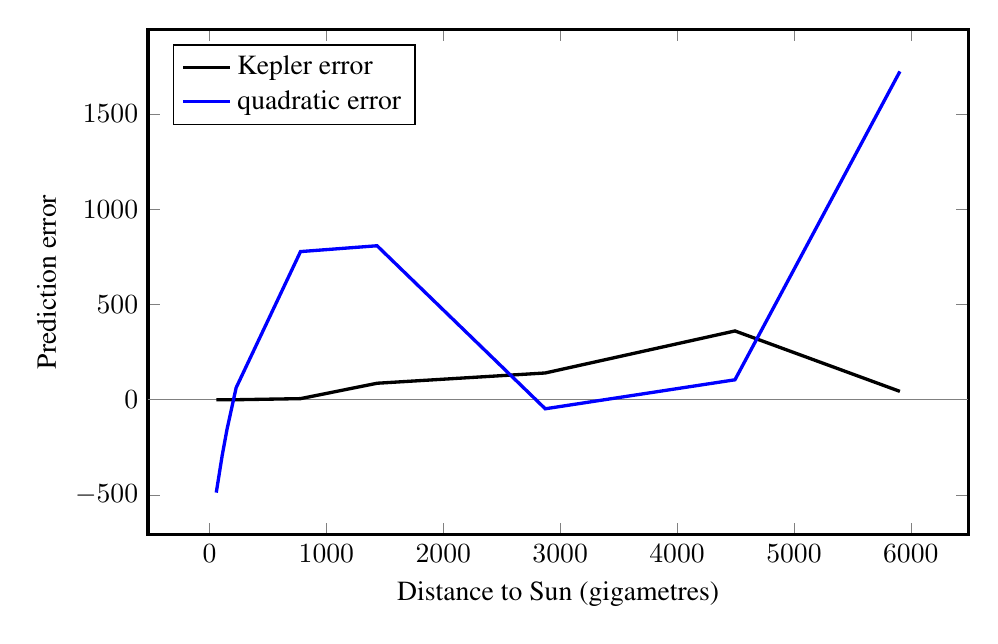
\begin{tikzpicture}
\tikzset{%%
  every mark/.append style={scale=1.0},%%
  scale=1.0%%
}
\pgfplotsset{%%
  every axis/.append style={font=\normalsize}%%
}
%%
\begin{axis}[%%
  axis line style=very thick,%%
  enlargelimits=true,%%
  height=8cm,%%
  legend cell align=left,%%
  legend pos=north west,%%
  plotStyle/.style={very thick,mark=none},%%
  width=12cm,%%
  %% x axis
  xlabel={\normalsize Distance to Sun~(gigametres)},%%
  xtick={0,1000,2000,3000,4000,5000,6000},%%
  xticklabels={$0$,$1000$,$2000$,$3000$,$4000$,$5000$,$6000$},%%
  %% y axis
  ylabel={\normalsize Prediction error},%%
  ytick={-500,0,500,1000,1500},%%
  yticklabels={$-500$,$0$,$500$,$1000$,$1500$},%%
  scaled y ticks=false,%%
  y tick label style=/pgf/number format/fixed%%
]
%%
%%
%% Horizontal line through origin.
\draw[gray,thin] ({rel axis cs:0,0}|-{axis cs:0,0}) -- ({rel axis cs:1,0}|-{axis cs:1,0});
%%
%%
%% The errors from Kepler's function.
\addplot[plotStyle,black] coordinates {
  (57.9, -0.061635843698795)
  (108.2, -0.052583685325061)
  (149.6, 0.022838307997574)
  (227.9, -0.284223816037297)
  (778.6, 5.42796064498543)
  (1433.5, 86.2080273900065)
  (2872.5, 140.15322669781)
  (4495.4, 360.723268177411)
  (5906.4, 43.4677343944495)
};
\addlegendentry{Kepler error}
%%
%%
%% The errors from the quadratic function.
\addplot[plotStyle,blue] coordinates {
  (57.9, -487.841084)
  (108.2, -294.062036)
  (149.6, -156.483204)
  (227.9, 62.6445160000002)
  (778.6, 777.324876000001)
  (1433.5, 808.0033)
  (2872.5, -47.8307000000023)
  (4495.4, 104.363915999995)
  (5906.4, 1722.97599599999)
};
\addlegendentry{quadratic error}
\end{axis}
\end{tikzpicture}

\end{document}
